\clearpage
\subsectionold{MSVC + \olly}
\myindex{\olly}

Попробуем этот же пример в \olly.
Загружаем, нажимаем F8 (\stepover) до тех пор, пока не окажемся в своем исполняемом файле,
а не в \TT{ntdll.dll}.
Прокручиваем вверх до тех пор, пока не найдем \main.
Щелкаем на первой инструкции (\TT{PUSH EBP}), нажимаем F2 (\IT{set a breakpoint}), 
затем F9 (\IT{Run}) и точка останова срабатывает на начале \main.

Трассируем до того места, где готовится адрес переменной $x$:

\begin{figure}[H]
\centering
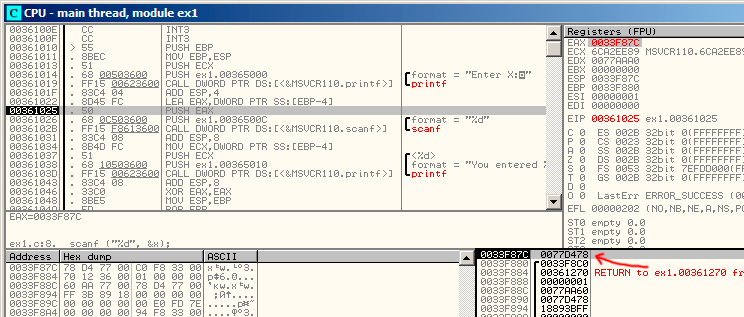
\includegraphics[scale=\FigScale]{patterns/04_scanf/1_simple/ex1_olly_1.png}
\caption{\olly: вычисляется адрес локальной переменной}
\label{fig:scanf_ex1_olly_1}
\end{figure}

На \EAX в окне регистров можно нажать правой кнопкой и далее выбрать \q{Follow in stack}.
Этот адрес покажется в окне стека.

Смотрите, это переменная в локальном стеке. Там дорисована красная стрелка.
И там сейчас какой-то мусор (\TT{0x6E494714}).
Адрес этого элемента стека сейчас, при помощи \PUSH запишется в этот же стек рядом.
Трассируем при помощи F8 вплоть до конца исполнения \scanf.
А пока \scanf исполняется, в консольном окне, вводим, например, 123:

\begin{figure}[H]
\centering
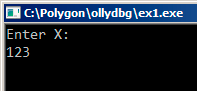
\includegraphics[scale=\NormalScale]{patterns/04_scanf/1_simple/ex1_olly_2.png}
\caption{Ввод пользователя в консольном окне}
\label{fig:scanf_ex1_olly_2}
\end{figure}

\clearpage
Вот тут \scanf отработал:

\begin{figure}[H]
\centering
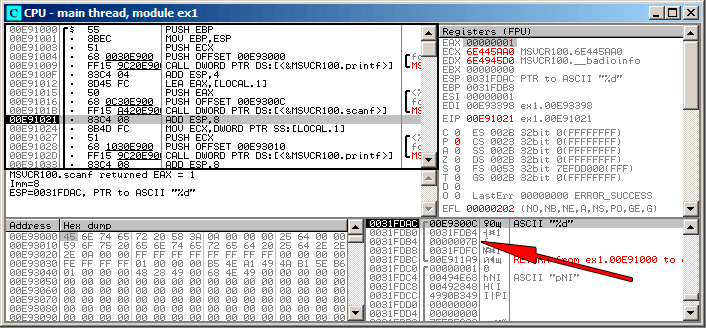
\includegraphics[scale=\FigScale]{patterns/04_scanf/1_simple/ex1_olly_3.png}
\caption{\olly: \scanf исполнилась}
\label{fig:scanf_ex1_olly_3}
\end{figure}

\scanf вернул 1 в \EAX, что означает, что он успешно прочитал одно значение.
В наблюдаемом нами элементе стека теперь \TT{0x7B} (123).

\clearpage
Чуть позже это значение копируется из стека в регистр \ECX и передается в \printf{}:

\begin{figure}[H]
\centering
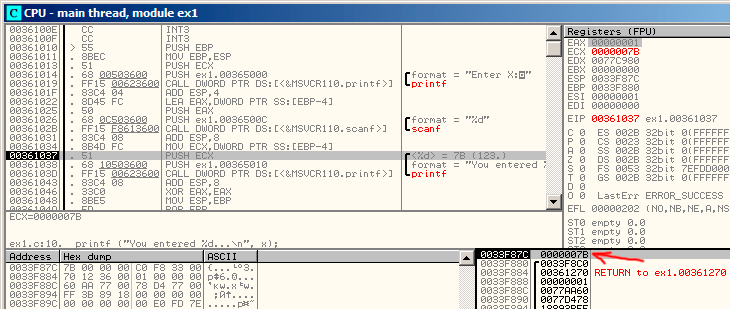
\includegraphics[scale=\FigScale]{patterns/04_scanf/1_simple/ex1_olly_4.png}
\caption{\olly: готовим значение для передачи в \printf}
\label{fig:scanf_ex1_olly_4}
\end{figure}
